Historii psaní dokumentů jsme si popsali v~minulé kapitole, nyní je čas popsat princip, kterým dokumenty vznikají. Vznik dokumentů také prochází
vývojem, ale tento vývoj přichází až v~poslední době s rozvojem informačních technologí.

Tvorba dokumentů by se dala rozdělit na dva různé přístupy.
První má za výsledek jeden soubor, který tvoří daný dokument a druhý pouze složí dokument z určitých částí.

Než si ovšem popíšeme tyto dva přístupy, je nutné se podívat, jak vlastně dokument vzniká. Nejdříve je nutné vytvořit návrh, pro který se také používá
označení draft. Tento draft je pouze základní obrys toho, co by měl výsledný dokument obsahovat. Pokud se na dokumentu podílí více autorů, je
tento draft kontrolován každým z nich. Z draftu se potom začne rozvíjet výsledný dokument, který se po dopsání předává ke kontrole korektorům,
kde se \mbox{kontroluje} pravopis a stylistika. Po konečné kontrole díla autorem či autory je dílo předá\-no distributorovi. Celý tento postup
je znázorněn na grafu. \ref{fig:linflow}

\begin{figure}[h]
    \centering
    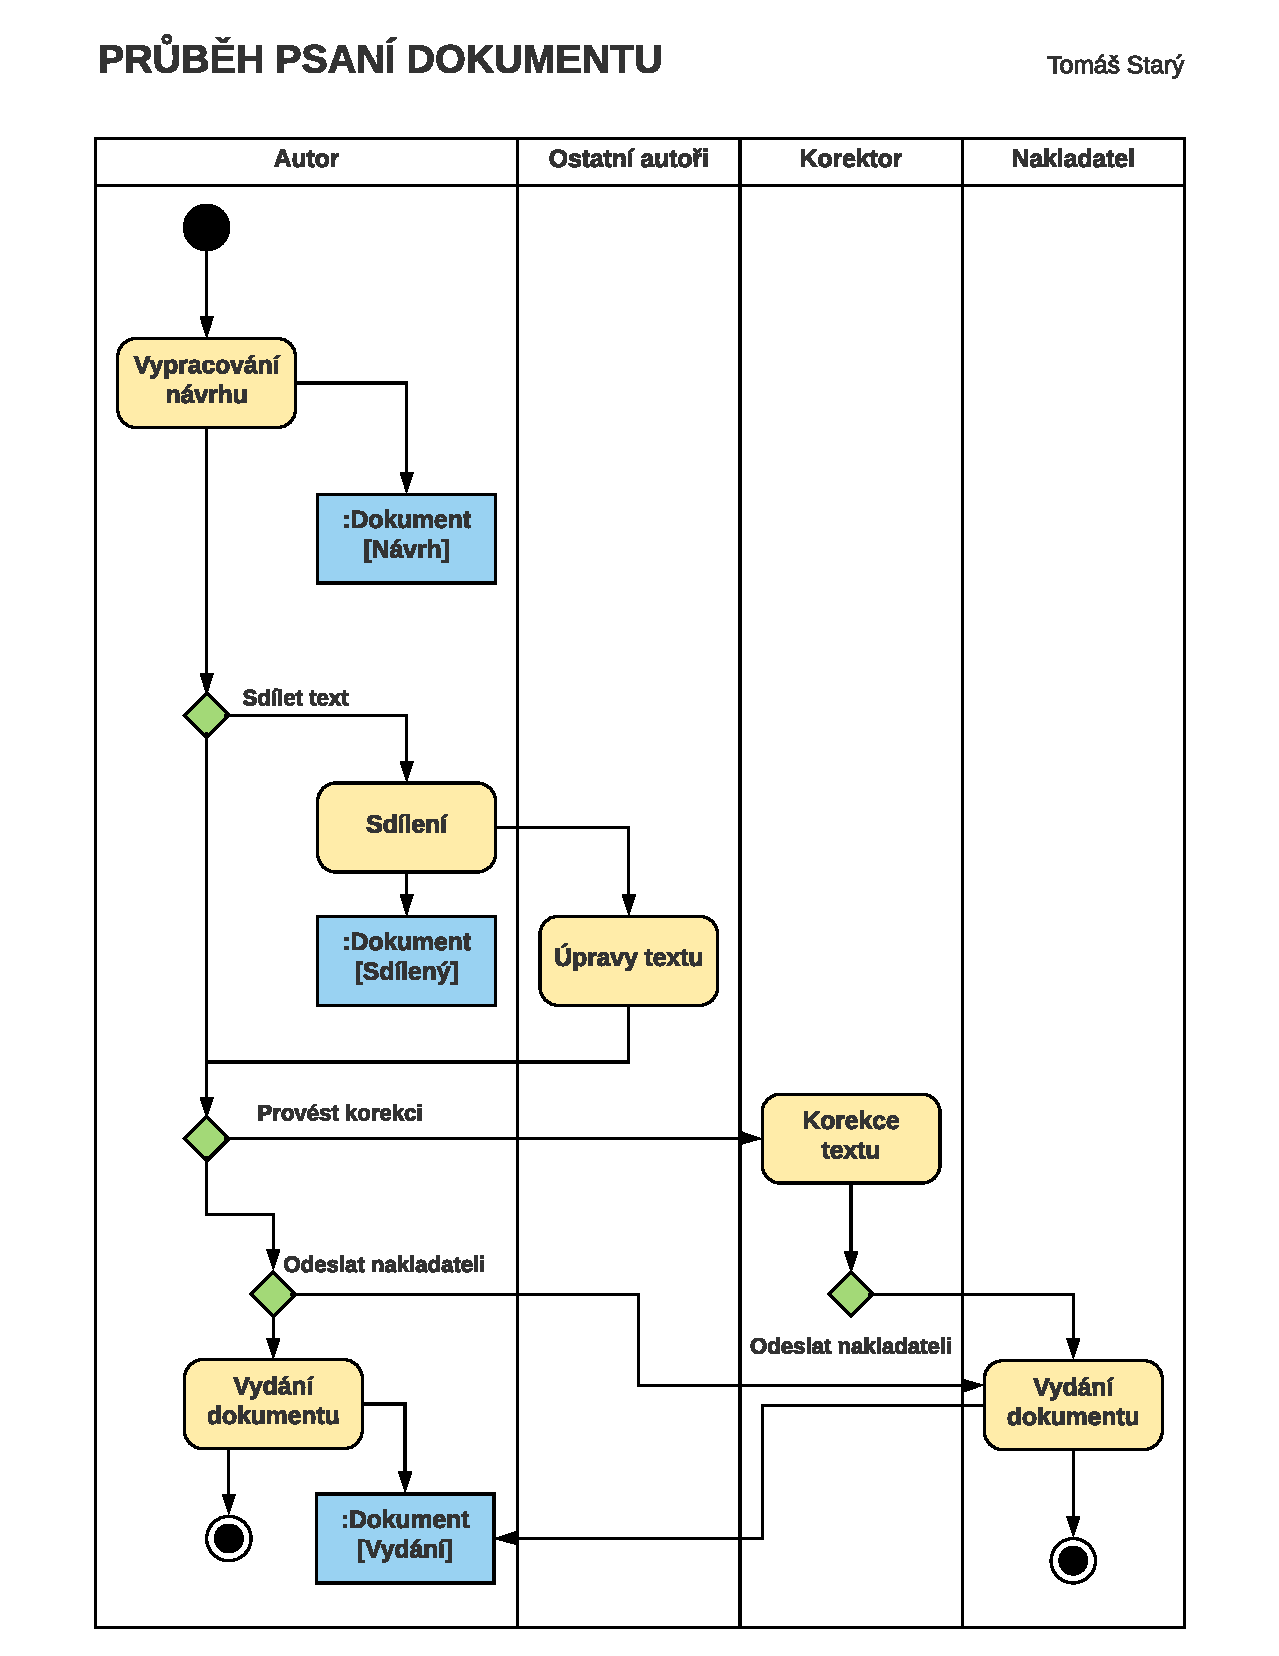
\includegraphics[width=\textwidth]{document.pdf}
    \caption{Průběh psaní dokumentu}
    \label{fig:linflow}
\end{figure}

\section{Monolitický přístup}

Monolitickým přístupem je myšleno to, že jednotlivé dokumenty jsou monolitické celky, jeden dokument je jeden celek. Pro představu, pokud si vezmeme ku příkladu
Word, o kterém už zaznělo něco v~kapitole o historii psaní dokumentů, vytvořením jednoho souboru s příponou .docx, jsme vytvořili jeden monolitický dokument a pokud jej
budeme chtít použít v~jiném dokumentu, budeme muset obsah tohoto souboru zkopírovat do nového souboru. Tento nový soubor bude obsahovat i náš původní dokument,
pokud se ovšem něco změní v~původním dokumentu, druhý dokument bude mít stále původní verzi. Toto poté přináší problémy, které byly již nastíněny v~úvodu této práce.

Výhodami monolitického přístupu jsou jednoduché zpracování jednoho\linebreak dokumentu. Není třeba jej dělit a je jednoduché jej sdílet i v~původním, nezpracovaném tvaru, kdy je
možné odeslat pouze jeden soubor. Nevýhody se hlavně projevují u větších textů, kdy může být nepřehledné orientování se v~jednom souboru a toto se ještě více
prohlubuje u~formátů, které nejsou jednoduché na čtení, pokud nejsou zpracovány například v~\gls{html} nebo \gls{xml}.

V~souvislosti se zmíněným formátem .docx, který je používaný hlavně programem Word z balíčku Office od firmy Microsoft, je třeba zmínit, že minimálně od verze 2016, je
možné rozdělit dokument na hlavní dokument a jeho části, které mohou být uchovávány odděleně. \cite{msWord} Toto řešení je ovšem citlivé na přesuny souborů
a není optimální.

\section{Modulární přístup}

Hlavní myšlenkou modulárních dokumentů je rozdělit dokument na jednotlivé moduly, tedy části textu, které je možné poté využít i v~jiných dokumentech. Jako příklad uvedu
tuto práci. Skladá se z jednotlivých kapitol. Tyto kapitoly jsou více či méně na sobě nezávislé a tudíž se dají rozdělit na jednotlivé moduly. Ovšem nemusíme tento
dokument dělit pouze podle kapitol, je možné jej rozdělit i na měnší části. S tímto dělením si ovšem musíme dát pozor, abychom dokument nerozdělili na moc malé části,
které potom samy o sobě ztratí smysl.

Jak nám toto pomůže zlepšit efektivitu psaní a rozšiřování dokumentů? Je potřeba si uvědomit, že pokud se k nám přídá nový člen týmu, který má spravovat naší
dokumentaci, je pro něj složité se orientovat v~jednom velkém monolitickém souboru. Pokud ovšem je možnost dokumentaci rozdělit
na části, je i pro nově příchozího člena týmu jednodušší zorientovat se v~upravované části a případně ji rozšířit. Pro lidi, kteří dokumentaci píšou již delší dobu, bude mimo jiné přínosné
nutnost držet se jednoho tématu, který může definovat daný modul a tím pádem držet konzistentnost obsahu textu. \cite{modularDocuments}

Výhodou modulárního přístupu mimo těch nastíněných v~přechozím odstavci, je možnost jednoduchého aktualizování textu, mezi vícero dokumenty, které sdílejí stejný modul. Také
tento způsob přináší možnost přehlednějšího verzování, kdy je možné procházet pouze změny v~jednotlivých modulech. Nevýhody jsou hlavně v krátkých a unikátních dokumentech,
kdy není ani žádoucí je rozdělovat do vícero souborů. Další nevýhodou je, že ne všechny formáty, které slouží k psaní textu, tuto metodu podporují (Markdown).
